%% The following is a directive for TeXShop to indicate the main file
%%!TEX root = ../diss.tex

\chapter{Chemical Exchange Saturation Transfer}
\label{ch:CEST}

\section{Preface}

\section{Introduction}

In the year 2000, Ward, Aletras, and Balaban published a seminal paper describing a new phenomenon called chemical exchange saturation transfer (CEST).
In fact, this effect had actually been used in MR spectroscopy for over 40 years before this discovery but under a slightly different name: magnetization or saturation transfer.
Since Ward et al. published their exciting results using exogenous agents to enhance the CEST affect, CEST-MRI has garnered significant attention as a method of generating contrast \emph{in vivo}~\cite{Sherry:2008jg}.
The CEST effect arises when magnetization is transferred through protons, between a saturated pool and an unsaturated pool.

\section{Theory}

In the context of conventional MR spectroscopy, chemical exchange occurs between protons on different chemical species and the exchange process is governed by basic forward and reverse rate constants.
Consider a system with two distinct pools of protons are able to undergo chemically exchange, for example protons from the surrounding water (Pool A) capable of exchanging with a proton on a molecule (Pool B).
Recall that when a spin $\frac{1}{2}$ particle (for e.g., a proton) is placed in a magnetic field, two possible energy states are possible (Fig~\ref{saturation}), one aligned with the magnetic field (low energy) and one aligned against the magnetic field (high energy).
The spins aligned with the magnetic field are in a lower energy state and thus, the probability of finding the nucleus in this state is slightly higher.
The probability of a spin aligned with (or against) the magnetic field is inversely related to the energy of the  state described by the Boltzmann distribution,

\begin{equation*}
P(E\uparrow) = Ce^{\frac{-E\uparrow}{k_b T}}
\end{equation*}

where C is a proportionality constant, T is the temperature of the system, and $k_b$ is the Boltzmann constant.
A magnetization vector arises from an excess population of spins in the lower energy state and this is the source of MR signal.
The strength of this magnetization vector can be temporarily reduced by the application of a low-power RF pulse (known as a saturation pulse) directed at one, or both of the proton pools.
If the saturation pulse leads to an equal population of spins in both energy states, the net magnetization becomes zero and the system is `saturated'~\cite{Sherry:2008jg}.
However, due to ongoing chemical exchange, both the high and low energy spins from the saturated pool transfer to the unsaturated pool (Fig~\ref{saturation}).
The exchange processes describing the transfer of spins between 1) the high energy spins in Pool A and B and 2) low energy spins in Pool A and B are modelled as two independent equilibria with a rate constant governing each process separately~\cite{Woods:2006cq}.
If a saturation pulse is applied on resonance at Pool A, the net result of chemical exchange on this system (over time) is a reduction in the number of Pool B spins in the lower energy state and an increase in the number of Pool B spins in the higher energy state.
Ultimately, this leads to decreased signal intensity in the Pool B as well.
Together, saturation, transfer, and chemical exchange make up the CEST effect.

\begin{figure}[htbp]
\begin{center}
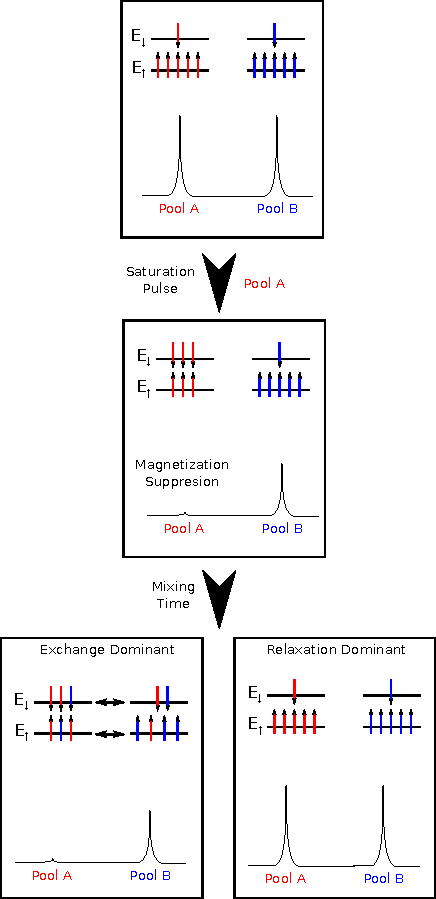
\includegraphics[width=0.4\textwidth]{cest/cest-images/cest_saturation.pdf}
\caption{\textbf{Summary of the CEST effect.} Initially two pools are considered, each with exchangeable protons.
The peaks correspond to the signal intensity from an image.
If a saturation pulse is applied with a saturation frequency at the resonance frequency of Pool A, the magnetization vector is decreased and signal intensity is suppressed.
Because of chemical exchange, the Pool B magnetization vector also decreases slightly.
If the system is dominated by relaxation (i.e.
if relaxation occurs as fast or faster than proton exchange) then the CEST effect is not observed the system recovers to its equilibrium state.
If the relaxation time is long relative to the exchange rate, a CEST effect is observed.
\newline \emph{\small{Image credit: adapted from Woods et al.~\cite{Woods:2006cq}}}}
\label{saturation}
\end{center}
\end{figure}
	
The CEST effect is only observed under specific conditions of exchange and relaxation.
At equilibrium, the spin population is distributed according to the Boltzmann distribution and the saturation pulse acts as a perturbation.
The longitudinal relaxation time (T$_1$) slowly counteracts this perturbation and if T$_1$ is short relative to the exchange rate (k$_{ex}$ describing proton transfer from Pool A to Pool B, the CEST effect is not observed~\cite{Woods:2006cq} and the system is dominated by relaxation (Fig.~\ref{saturation}).
A further criteria is that the exchange process must be slow relative to the NMR time scale,
	
	\begin{equation}
		\Delta \omega \geq k_{eq}
	\end{equation}

where $\Delta \omega$ is the difference between the Larmor frequencies of the two pools.
By saturating the bulk/free water pool, the magnetization from this pool is decreased and by saturation transfer, magnetization from the other pool also decreases.
From an imagine perspective, the net result is an overall darkening coupled with an increase in contrast as the difference between the two pools is increased.
Typically, negative contrast is not preferred in MR imaging because the human eye can more easily discriminate between a slight increase in image intensity than a similar decrease.
However, generation of this contrast can easily be controlled by turning off the saturation pulse prior to imaging.
Thus, data can be acquired with and without saturation, and post-processing techniques can be used to generate a `difference-image' consisting of positive contrast.

\subsection{APT-CEST}     

While there are several types of CEST contrasts available, in this
work we will focus our attention just on one subset, amide proton transfer or APT.
APT refers specifically to the chemical exchange between bulk-water protons and amide groups (-NH) of endogenous mobile peptides and proteins as it is most relevant for tumours~\cite{Togao:2013gn}.
The concentration of these mobile peptides and proteins is in the millimolar range and that has thusfar limited their utility to be considered a viable target for clinical diagnosis or prognosis, at least using MRI.
However due to the saturation transfer effect, APT imaging can be used to elucidate the presence of these mobile peptides and proteins~\cite{Zhou:2003cc}.
The APT effect arises when the amide groups on the protein backbones exchange with water protons after a saturation pulse directed at around 3.5 ppm with respect to water~\cite{vanZijl:2003in}.
Interestingly, the side chains of these same proteins and peptides comprising mostly the amino acids glutamine and asparagine that
resonate at about 2 ppm~\cite{vanZijl:2003in}.
Another potential contribution to the APT effect are the nucleosides that make up DNA and RNA molecules (nucleotides - adenosine, guanine, cytosine, uracil, thymine -  just without a phosphate group) but in their normal forms, the base pairs are hydrogen bonded so the exchange rates of those protons is very low (k$_{ex}$ < 0.01 s$^{-1}$) and these protons exchange very slowly with water.
When these DNA and RNA base pairs are caused to break down, denature, or separate, the labile protons are exposed and the concentration of exchageable protons increases resulting in a higher APT signal.
One can hypothesize that a treatment resulting in direct DNA damage and protein denaturation to expose additional hydrogens that could exchange with water would result in an APT signal increase in tumours.

Recently, CEST has been proposed to assess several the efficacy of several therapies and in this study we extend this work by first assessing the baseline variability of the APT effect, and then evaluate the efficacy of two treatments that may result in DNA damage (10Gy dose of whole-body radiation), as well as rapid loss of perfusion ultimately resulting in large-scale tumour necrosis (chemotherapy combretastatin)~\cite{Maxwell:2002da}.
Combretastatin is a a vascular targeting drug Combretastatin A-4 phosphate (CA4P) that has been shown to have both a strong acute effect at low dose, and a long term effect at high dose~\cite{Maxwell:2002da}.
To study the effect of these treatments on the APT CEST signal, an experiment was conducted to first assess the baseline repeatability (test-retest on subsequent days) of the APT CEST signal, followed by a treatment prior to the last imaging session.

\section{Development}

\subsection{MR Sequences}

\subsection{Phantom Work}

\subsection{Quantification \& Fitting}

\section{Methods}

\subsection{Animals}: NOD/SCID mice were implanted with a murine squamous cell carcinoma (SCCVII) on the left flank and tumours were allowed to grow until they reached 500mm$^3$.


\subsubsection{Experiment 1: CEST Controls + CA4P (CestS1)}

Animals were imaged daily for three days.
Then, 7 of those mice were injected i.p. with 120$\mu$L of CA4P at a dose~\cite{Maxwell:2002da} of 80 mg/kg and imaged 24 hrs later.


\subsubsection{Experiment 2: CEST + 10Gy (CestS)}

5 mice received a 10Gy dose of radiation and were imaged 96 hours later (CestS2).


\subsubsection{Experiment 3: CEST + 40Gy (CestS3)}

5 mice received 40Gy dose of radiation and imaged 

Wednesday November 16, 2016 5 mice were irradiated with 40Gy but left at BCCRC for monitoring.
Mice were imaged and euthanized on Nov.
22nd, 2016.

\subsection{Imaging}

Imaging was performed using a 7T small animal scanner.
CEST scans were acquired using an EPI-based imaging scheme and continuous-wave saturation with B$_1$=1.0$\mu$T for 10s at each saturation frequency offset.
Spatial resolution of the CEST scan was 0.5 mm in-plane with a 1.5 mm slice thickness.
80 offset frequencies were acquired ranging from -20 to +20 ppm with a higher spectral resolution near peaks of interest.
Total scan time for the CEST sequence was 27 minutes.

\subsection{Histology}

\textbf{Histology:} Following the last imaging session, animals were injected with 50$\mu$L of the perfusion dye carbocyanine 5 minutes prior to sacrifice and the tumours were immediately excised and frozen.
Sequential sections 10$\mu$m thick were obtained every 0.5 mm and analysed to identify the fraction of perfused vessels and necrosis.
Sections were stained with TUNEL/CASPASE to mark apoptosis and CD31 to mark blood vessels.


\section{Results}

Figures~\ref{mainCest} \&~\ref{cestFractions} summarize the main results of the study, and the conclusions are summarized here:

\begin{enumerate}
\item While some changes in a subset of tumours can be observed in Figure~\ref{mainCest}, the tumour pixel distributions in the control groups are not statistically significantly different from the CA4P treatment group (red)

\item Histological evidence also did not point to a strong effect of treatment compared to the control groups~\ref{cestFractions}

\item Consequently, comparisons of the amine and amide peak sizes to histological fraction did not yield any conclusive correlations.

\end{enumerate}

\begin{figure}[htbp]
\begin{center}
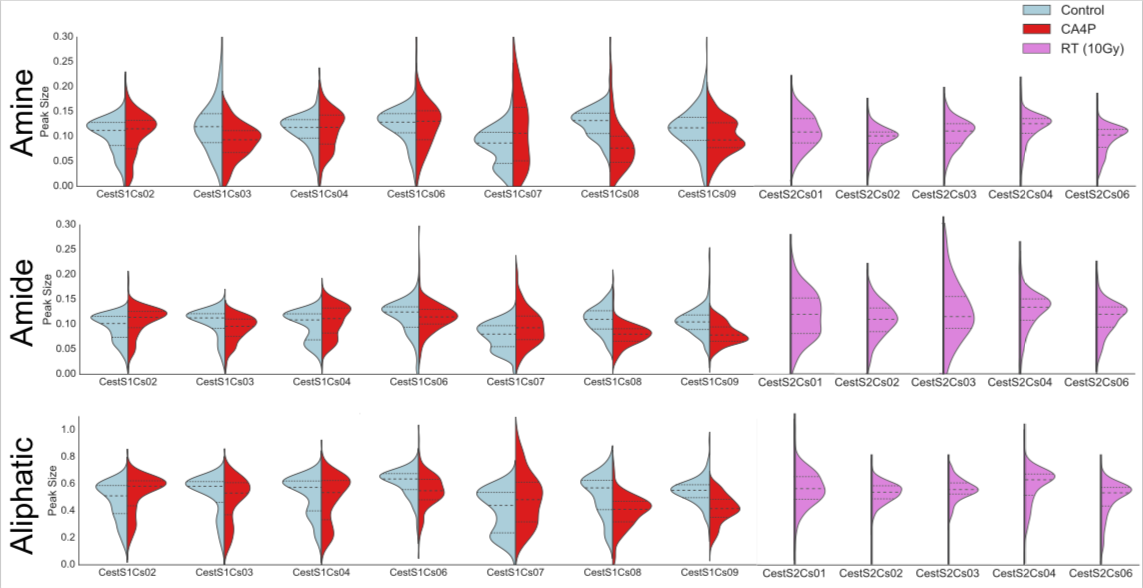
\includegraphics[width=\textwidth]{cest/cest-images/cest_Violinplots.png}
\caption{Peak-size (width x amplitude of peak) voxel distributions of every animal are shown as violin-plots for each of the three peaks of interest (amine at $\approx$2.2 ppm, amide at $\approx$3.5 ppm, and aliphatic at -3.5 ppm).
Colours represent the distribution at each treatment group: control (light blue), 24h post CA4P treatment (red), and 96h post 10Gy RT (violet).
Dashed lines within each half-violin corresponds to the median, and the dotted lines indicate the first and third quartiles.}
\label{mainCest}
\end{center}
\end{figure}

\begin{figure}[htbp]
\begin{center}
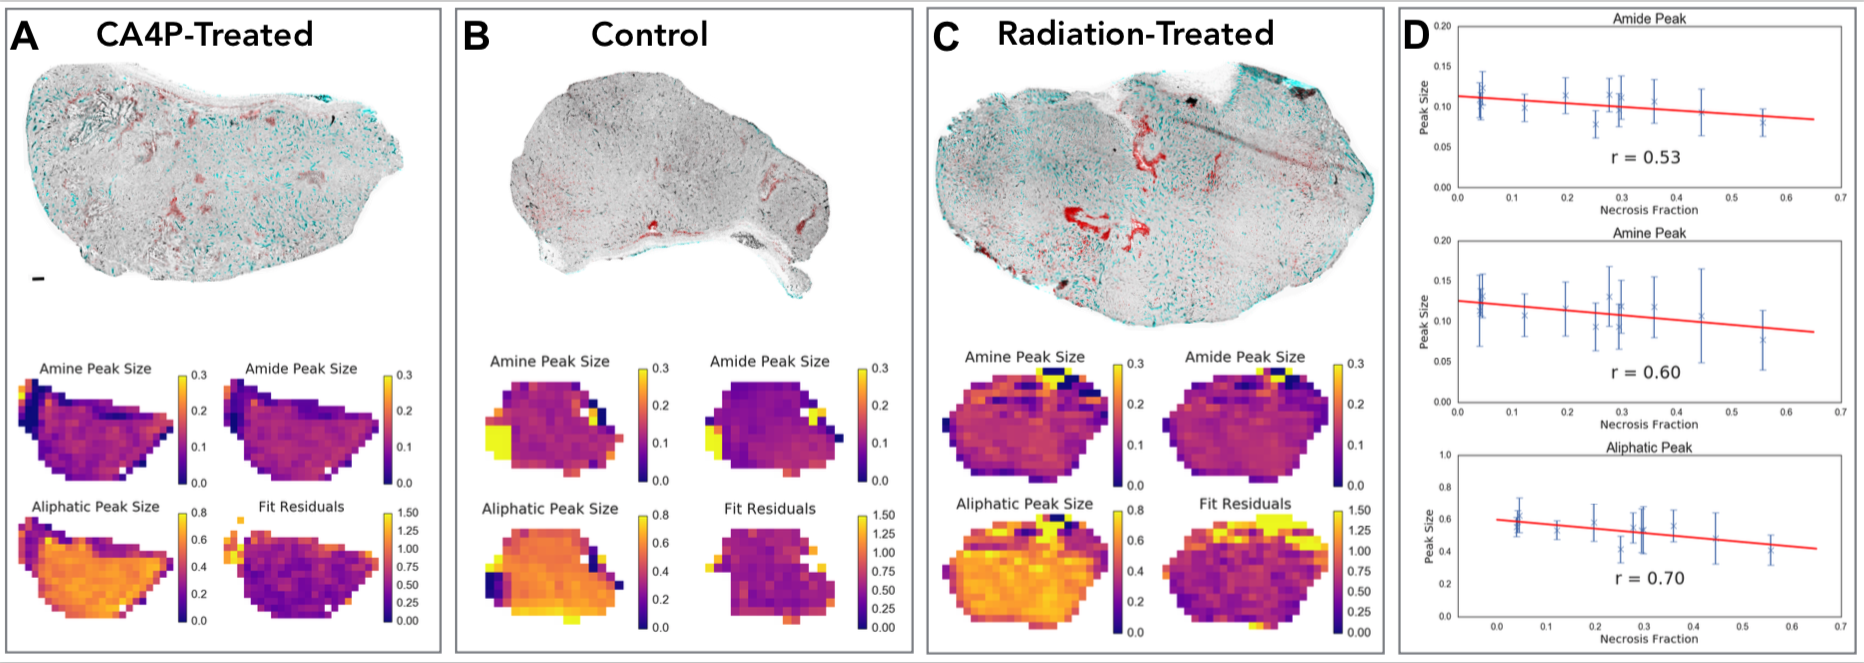
\includegraphics[width=\textwidth]{cest/cest-images/cest_RTstudy}
\caption{Representative histology sections are shown for each of the groups (A-C), as well as CEST parameter maps of a similar slice in the tumour.
CEST peak-size maps are shown for the amine, amide, aliphatic peaks as well as the fit residuals for each of the three groups.
The `fit-residual' maps were used to exclude voxels where fit quality was poor.
Necrosis fractions were calculated from the histology sections across all animals and treatment groups and plotted against the amine, amide, and aliphatic peak-sizes; r-values on the plots indicate the correlation coefficient.}
\label{cestFractions}
\end{center}
\end{figure}

%\section{Discussion}

%\section{Conclusions}


\endinput

Any text after an \endinput is ignored.
You could put scraps here or things in progress.
